% Bremen Big Data Challenge - Edition 2019
%
% Data Analysis Competition
%
% Team `gentleman`
%
% Created on March 10, 2019
%
% Authors:
%   Gari Ciodaro <g.ciodaroguerra@jacobs-university.de>
%   Diogo Cosin <d.ayresdeoliveira@jacobs-university.de>
%   Ralph Florent <r.florent@jacobs-university.de>
%
% Contents block for the documentation
%
% 1) Introduction
% 2) Background of the data (data description)
% 3) Data preprocessing
% 4) Data exploitation
% 5) Data Analysis
% 6) Conclusion / Results
% 7) References / Bibliography

% ==============================================================================
% START: Methods, Results, Discussions, Conclusion
% ==============================================================================

\section{Background of the Data}
\subsection{Data Source}

Provided by \emph{"The Bremen Big Data Challenge 2019" Organizers}, the collected data are based on
daily athletic movements \parencite{bbdc}. Using wearable sensors above and below the knee (See
Figure \ref{fig:sensor-placement}) of the individual (athletic), a dataset of 19 individuals, mainly
identified as \emph{subjects}, has been recorded. And as the competition requires, the data of 15
out of the total number of subjects are used as the training dataset and the remaining part as the
testing dataset. The dataset is publicly available online on the official website:
\href{https://bbdc.csl.uni-bremen.de/images/2019/bbdc_2019_Bewegungsdaten_mit_referenz.zip}{BBDC} or
by simply browsing through the following URL: \emph{https://bbdc.csl.uni-bremen.de/index.php/2019h/28-aufgabenstellung-2019}.

\begin{figure}
    \centering
    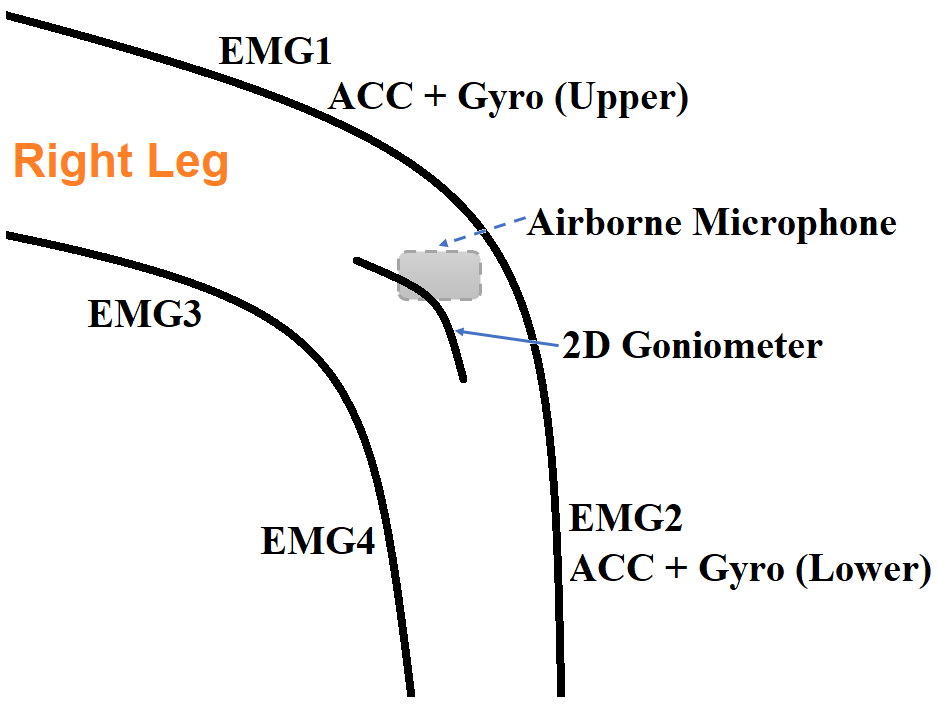
\includegraphics[scale=0.33]{sensor-placement.png}
    \caption{Wearable sensor placement for data measurements. (source: part of the provided data)}
    \label{fig:sensor-placement}
\end{figure}

\subsection{Description and Format}

The data comprise the following 22 movements:
\begin{itemize}
    \item Race ('run')
    \item Walking ('walk')
    \item Standing (standing)
    \item Sitting ('sit')
    \item Get up and sit down ('sit-to-stand', 'stand-to-sit')
    \item Up and down stairs ('stair-up', 'stair-down')
    \item Jump on one or both legs ('jump-one-leg', 'jump-two-leg')
    \item Run left or right ('curve-left-step', 'curve-right-step')
    \item Turn left or right on the spot, left or right foot first ('curve-left-spin-Lfirst',
    'curve-left-spin-Rfirst', 'curve-right-spin-Lfirst', 'curve-right- spin-Rfirst ')
    \item Lateral steps to the left or right ('lateral-shuffle-left', 'lateral-shuffle-right')
    \item Change of direction when running to the right or left, left or right foot first
    ('v-cut-left-left', 'v-cut-left-right', 'v-cut-right-left', 'v-cut' right-Rfirst ')
\end{itemize}

The entire data are available as CSV files, or Comma-Separated Values, and partitioned as training and
testing data, respectively represented by the "\textbf{\emph{train.csv}}" and the "\textbf{\emph{challenge.csv}}"
files. Starting with the training dataset file (\textbf{\emph{train.csv}}), it contains
\emph{UTF-8}\footnote{Unicode Transformation Format, extended ASCII, variable-width encoding.}
character-encoded, line-wise plain texts, whose first line identifies the feature names
followed by the feature values. This file contains a total of 6402 lines, which include both the
feature names and the feature values. The feature names are \textit{Subjects}, \textit{Datafile}, \textit{Label},
and the feature values map respectively each feature name. For instance, the first feature values of
the file are: \textit{Subject02}, \textit{ \path{Subject02 / Subject02_Aufnahme002.csv}},
\textit{stand-to-sit}. Table \ref{table:train-data} illustrates a lightweight version of the
data partition of the training dataset file.

\begin{table}
    \begin{center}
        \begin{tabular}{||c | c | c||}
            \hline % Table headers
            \textbf{Subjects} & \textbf{Datafile} & \textbf{Label} \\ [0.5ex]
            \hline \hline % Table body (row-wise contents)
            Subject02 & \path{Subject02 / Subject02_Aufnahme000.csv} & \textit{curve-left-step} \\
            \hline
            Subject02 & \path{Subject02 / Subject02_Aufnahme001.csv} & \textit{curve-left-step} \\
            \hline
            Subject02 & \path{Subject02 / Subject02_Aufnahme002.csv} & \textit{stand-to-sit} \\
            \hline
            ... & ... & ... \\
            \hline
            Subject19 & \path{Subject19 / Subject19_Aufnahme438.csv} & \textit{curve-right-step} \\
            \hline
            Subject19 & \path{Subject19 / Subject19_Aufnahme439.csv} & \textit{curve-right-spin-Rfirst} \\
            \hline
        \end{tabular}
        \caption{Tabular visualization of the "\textbf{\emph{train.csv}}" dataset}
        \label{table:train-data}
    \end{center}
\end{table}

Similarly, the testing dataset file (\textbf{\emph{challenge.csv}}) is formatted using the same structure
with the exception of the \textit{Label} column, which is unknown and marked with an \emph{X}.
The datafile contains a total of 1739 lines counting both the feature names and feature values.
Table \ref{table:test-data} displays a lightweight version of the data partition of the testing
dataset file.

\begin{table}
    \begin{center}
        \begin{tabular}{||c | c | c||}
            \hline % Table headers
            \textbf{Subjects} & \textbf{Datafile} & \textbf{Label} \\ [0.5ex]
            \hline \hline % Table body (row-wise contents)
            Subject01 & \path{Subject01 / Subject01_Aufnahme000.csv} & \textit{X} \\
            \hline
            Subject01 & \path{Subject01 / Subject01_Aufnahme001.csv} & \textit{X} \\
            \hline
            Subject01 & \path{Subject01 / Subject01_Aufnahme002.csv} & \textit{X} \\
            \hline
            ... & ... & ... \\
            \hline
            Subject15 & \path{Subject15 / Subject15_Aufnahme438.csv} & \textit{X} \\
            \hline
            Subject15 & \path{Subject15 / Subject15_Aufnahme439.csv} & \textit{X} \\
            \hline
        \end{tabular}
        \caption{Tabular visualization of the "\textbf{\emph{challenge.csv}}" dataset}
        \label{table:test-data}
    \end{center}
\end{table}

\noindent
\textbf{Important}: Recalling that the dataset is divided into training and testing data, the subjects
"\emph{Subject01, Subject10, Subject14, Subject15}" are the selected ones that are used as testing
data to assess the solutions. Note the difference in the starting and ending rows of Tables
\ref{table:train-data} and \ref{table:test-data}.

As observed in both Tables \ref{table:train-data} and \ref{table:test-data}, each line corresponds
to a recording of a movement. The columns have the following meanings:
\begin{itemize}
    \item \textbf{\emph{Subject}}: The ID of the subject
    \item \textbf{\emph{Datafile}}: Path of the file containing the sensor data for this recording. For each subject,
    there is a folder in which individual data files contain the sensor data for individual motion
    recordings.
    \item \textbf{\emph{Label}}: The movement that was recorded
\end{itemize}

Particularly, the \emph{Label} column of the testing dataset contains repeatedly the letter "\textit{X}"
to indicate that this value is not present. That is, at the time of submitting solutions, the submission should
exactly match the testing data, where each \emph{X} will be replaced by a label. This label corresponds to the
classification result of a specific movement. It is important that the spelling (including upper / lower
case) of the textual labels matches exactly the spelling of the labels in the training data.

As mentioned above, the datafiles are references to other CSV files. For example, the path file
\path{Subject02 / Subject02_Aufnahme000.csv} is a CSV file itself within a folder named \emph{Subject02}
located in the root path (i.e., the current directory of the downloaded zip files). The CSV file itself
is dataset with a proper format. Basically, the file has a set of comma-separated numbered-values
that looks like this: \textit{32688,32224,32991,32609,32790,33048,37168,34610,27374,29068,29264,
28408,31784,28133,29295,29244,33216,37140,34736}.

Each line represents the sensor values measured at one time (sampled at 1000 Hz). The columns
represent the individual wearable sensors recording the human activities (see Figure \ref{fig:sensor-placement}):

\begin{enumerate}
    \item EMG1
    \item EMG2
    \item EMG3
    \item EMG4
    \item Airborne
    \item ACC upper X
    \item ACC upper Y
    \item ACC upper Z
    \item Goniometer X
    \item ACC lower X
    \item ACC lower Y
    \item ACC lower Z
    \item Goniometer Y
    \item Gyro upper X
    \item Gyro upper Y
    \item Gyro upper Z
    \item Gyro lower X
    \item Gyro lower Y
    \item Gyro lower Z
\end{enumerate}

% source is needed
The size of the CSV datafiles vary inappropriately. That is, in most cases, due to inaccurate measurements,
random initialization states, mechanical flaws, computational and processing cost, and so on.

\section{Data Preprocessing}

\section{Data Exploitation}

\section{Data Analysis}

\section{Results and Discussions}

\section{Conclusion}

% ==============================================================================
% START: Methods, Results, Discussions, Conclusion
% ==============================================================================